\chapter{THE REVERSE MAPPING PROBLEM}
\thispagestyle{plain}

\label{ReverseMapping}

The reverse-mapping problem is the problem of defining a function $f^{-1}$ that maps a system-level configuration $\mathbf y$ onto a solution space $\hat{\mathbf S}$ that represents all possible configurations that would have the system exhibit $\mathbf y$:
   \[ f^{-1}(\mathbf y) \rightarrow \hat{\mathbf S}. \]
Every configuration $\hat {\mathbf x} \in \hat {\mathbf S}$ should satisfy the constraint $f(\hat{\mathbf x}) \approx \mathbf y$, where $f$ is the forward mapping.
That is, $\hat{\mathbf S}$ contains all the points that would predict $\mathbf y$ in the forward mapping.

In this chapter, I give details of how \fw approaches the solution to this problem, in general, then delves deeper into actual implementations of the solution.
Then, I discuss evaluation criteria for implementations of reverse-mapping problem solutions.

\section{The \fw Approach}

The general approach taken by \fw for solving the reverse-mapping problem is similar to the \fw forward-mapping solution approach.
First, the different system-level properties are split into sub-problems.
Next, solution spaces for each sub-problem are constructed with a forward-mapping inversion technique.
Finally, each solution subspace is recombined to produce the space of configurations that will produce the provided system-level property.

Much like the forward-mapping solution, $\mathbf y$ is split into subspaces to simplify the problem:
\[ \mathbf y = \{y_0, y_1, \ldots, y_{|\mathbf y|}\}. \]
The solution space is split up in a similar manner:
\[ \hat{\mathbf S} = \{\hat S_0, \hat S_1, \ldots, \hat S_{|\mathbf S|}\}. \]
By performing this split, each forward mapping can be inverted independently:
\[ f^{-1}_i(y_i) \rightarrow \hat S_i. \]

Recombining the individual $\hat S_i$ into $\hat{\mathbf S}$ is not as simple as recombining individual $\hat y_i$ into $\hat{\mathbf y}$ in the forward-mapping solution.
Since each solution space represents which configurations satisfy a particular system-level requirement, the solution space $\hat{\mathbf S}$ is the intersection of all these spaces:
\[ \hat{\mathbf S} = \hat S_0 \cap \hat S_1 \cap \ldots \cap \hat S_{|\mathbf S|}.\]
All points at the intersection of these spaces should satisfy all system-level properties at once.

The nature of the solution spaces vary from approach to approach.
In the approaches used by \fw, they are represented as a collection of discrete subspaces, discrete exemplar points, sets of functions, or linear combinations.


\section{Approaches}

I have devised and evaluated a number of different approaches for solving the reverse-mapping problem in this dissertation research.
This section enumerates these approaches.
Although each the approaches are quite different, they all \textit{invert} a solution to the forward-mapping problem.
That is, they use the forward mapping to develop the reverse mapping, instead of learning the reverse mapping directly.
This has the benefit that the reverse-mapping solutions are agnostic to the regression method used to learn the forward mapping.

Each approach is follows a different technical process, but all query the forward mapping for points instead of using the original data set.
Most approaches conform to the assumption stated in Chapter \ref{ForwardMapping}: The Forward-Mapping Problem that all the system-level properties can be analyzed independently.
Every approach has a different method for intersecting the different solution spaces to find a solution space that satisfies all system-level properties at once.

Each approach has different computational and space complexity.
The expectations for each method and the situations in which they are optimal vary from domain to domain and from query to query.

The first two approaches discussed in this section, \textit{Thresholding} and \textit{Regression} / \textit{Interpolation} / \textit{Intersection}, conform to the theoretical framework outlined above.
Two other approaches are labeled as alternatives, as they do not follow the framework exactly, but perform a similar task.
In the final subsection, I discuss the special case in which the system-level property is a binary value (i.e., the forward mapping is classification).
Throughout this section, I use the NetLogo Fires ABM\footnote{More on the Fires model is discussed in Section \ref{sec:Fires}} as an example.
The Fires domain is simple, but has solution spaces that are easy to visualize.
Other domains, such as Wolf Sheep Predation, have to many dimensions to make graphing possible.
The arguments made with the aid of the Fires domain scale to larger dimensions.

\subsection{Thresholding}

\subsection{Regression/Interpolation/Intersection}

\subsubsection{Regression}
% smooths the plot, builds knots for use in interpolation
% knots are the corners of a hypercube
% this is preprocessing

%example fires:

\subsubsection{Interpolation}
% requirements for interpolation

\subsubsection{Intersection}


\begin{figure}[ht]
\centering
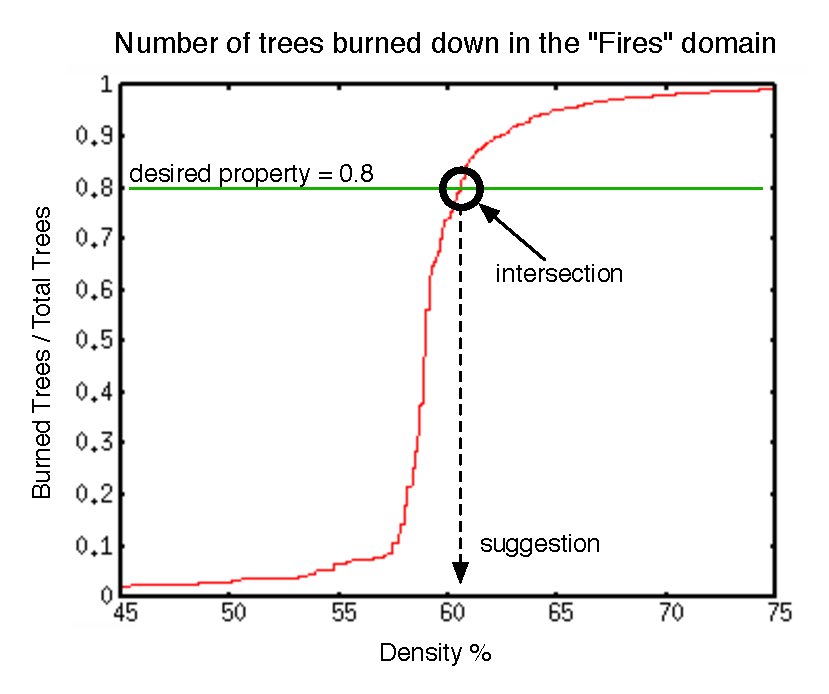
\includegraphics[scale=.66666667]{images/firespace-intersection.pdf}
\caption{An illustration of using surface-to-surface intersection to solve the reverse-mapping problem in the NetLogo Fires domain.}
\label{fig:fires-inter}
\end{figure}




\subsection{Alternative: Optimization}

\subsection{Alternative: Functional Inversion}

\subsection{Special Case: Classification}


\section{Using Reverse Mappings}




\section{Evaluation Criteria}

\subsection{Time Required for Preprocessing}

\subsection{Time Required for Querying}

\subsection{Accuracy of the Reverse Mapping}


\section{Summary}




